\chapter{Code Structure Overview}
%.
This TIEGCM code structure part is adapted from a document which can be found 
at the TIEGCM website http://www.hao.ucar.edu/modeling/tgcm/ under documentation
"TIEGCM Code Structure Flowchart (Documentation section of the Download page)".
The version on the web has hyperlinks included.
%
\begin{figure}
  \centering
  \includegraphics[scale=0.7,angle=-90.]{./tex_plot/code_1.ps}
  \caption{TIEGCM Code Structure
      Contents}
   \label{fig:code_1}
\end{figure}
%
\begin{figure}
  \centering
  \includegraphics[scale=0.7,angle=-90.]{./tex_plot/code_2.ps}
  \caption{\src{main}: TIEGCM main}
   \label{fig:code_2}
\end{figure}
%
%
\begin{figure}
  \centering
  \includegraphics[scale=0.7,angle=-90.]{./tex_plot/code_3.ps}
  \caption{\src{init}: model initialization}
   \label{fig:code_3}
\end{figure}
%
\begin{figure}
  \centering
  \includegraphics[scale=0.7,angle=-90.]{./tex_plot/code_4.ps}
  \caption{\src{advance}: advance model time}
   \label{fig:code_4}
\end{figure}
%
\begin{figure}
  \centering
  \includegraphics[scale=0.7,angle=-90.]{./tex_plot/code_5.ps}
  \caption{\src{dynamics}: dynamics and chemistry drivers}
   \label{fig:code_5}
\end{figure}
%
\begin{figure}
  \centering
  \includegraphics[scale=0.7,angle=-90.]{./tex_plot/code_6.ps}
  \caption{\src{aurora}: aurora parameterization}
   \label{fig:code_6}
\end{figure}
%
\begin{figure}
  \centering
  \includegraphics[scale=0.7,angle=-90.]{./tex_plot/code_7.ps}
  \caption{\src{oplus}: $O^+$ calculation}
   \label{fig:code_7}
\end{figure}
%
\begin{figure}
  \centering
  \includegraphics[scale=0.7,angle=-90.]{./tex_plot/code_8.ps}
  \caption{\src{dynamo}: calculation of electric potential}
   \label{fig:code_8}
\end{figure}
%
\begin{figure}
  \centering
  \includegraphics[scale=0.7,angle=-90.]{./tex_plot/code_9.ps}
  \caption{minor species composition}
   \label{fig:code_9}
\end{figure}
%
\begin{figure}
  \centering
  \includegraphics[scale=0.7,angle=-90.]{./tex_plot/code_10.ps}
  \caption{calculation of minor species}
   \label{fig:code_10}
\end{figure}
%
\begin{figure}
  \centering
  \includegraphics[scale=0.7,angle=-90.]{./tex_plot/code_11.ps}
  \caption{major species composition}
   \label{fig:code_11}
\end{figure}
%
\begin{figure}
  \centering
  \includegraphics[scale=0.7,angle=-90.]{./tex_plot/code_12.ps}
  \caption{\src{duv}: calculation of neutral horizontal winds}
   \label{fig:code_12}
\end{figure}
%
\begin{figure}
  \centering
  \includegraphics[scale=0.7,angle=-90.]{./tex_plot/code_13.ps}
  \caption{output structure}
   \label{fig:code_13}
\end{figure}
%
\begin{figure}
  \centering
  \includegraphics[scale=0.7,angle=-90.]{./tex_plot/code_14.ps}
  \caption{filtering in TIEGCM}
   \label{fig:code_14}
\end{figure}
%
\begin{figure}
  \centering
  \includegraphics[scale=0.7,angle=-90.]{./tex_plot/code_15.ps}
  \caption{\src{dt}: calculation of neutral temperature}
   \label{fig:code_15}
\end{figure}
